
% Default to the notebook output style

    


% Inherit from the specified cell style.




    
\documentclass[11pt]{article}

    
    
    \usepackage[T1]{fontenc}
    % Nicer default font (+ math font) than Computer Modern for most use cases
    \usepackage{mathpazo}

    % Basic figure setup, for now with no caption control since it's done
    % automatically by Pandoc (which extracts ![](path) syntax from Markdown).
    \usepackage{graphicx}
    % We will generate all images so they have a width \maxwidth. This means
    % that they will get their normal width if they fit onto the page, but
    % are scaled down if they would overflow the margins.
    \makeatletter
    \def\maxwidth{\ifdim\Gin@nat@width>\linewidth\linewidth
    \else\Gin@nat@width\fi}
    \makeatother
    \let\Oldincludegraphics\includegraphics
    % Set max figure width to be 80% of text width, for now hardcoded.
    \renewcommand{\includegraphics}[1]{\Oldincludegraphics[width=.8\maxwidth]{#1}}
    % Ensure that by default, figures have no caption (until we provide a
    % proper Figure object with a Caption API and a way to capture that
    % in the conversion process - todo).
    \usepackage{caption}
    \DeclareCaptionLabelFormat{nolabel}{}
    \captionsetup{labelformat=nolabel}

    \usepackage{adjustbox} % Used to constrain images to a maximum size 
    \usepackage{xcolor} % Allow colors to be defined
    \usepackage{enumerate} % Needed for markdown enumerations to work
    \usepackage{geometry} % Used to adjust the document margins
    \usepackage{amsmath} % Equations
    \usepackage{amssymb} % Equations
    \usepackage{textcomp} % defines textquotesingle
    % Hack from http://tex.stackexchange.com/a/47451/13684:
    \AtBeginDocument{%
        \def\PYZsq{\textquotesingle}% Upright quotes in Pygmentized code
    }
    \usepackage{upquote} % Upright quotes for verbatim code
    \usepackage{eurosym} % defines \euro
    \usepackage[mathletters]{ucs} % Extended unicode (utf-8) support
    \usepackage[utf8x]{inputenc} % Allow utf-8 characters in the tex document
    \usepackage{fancyvrb} % verbatim replacement that allows latex
    \usepackage{grffile} % extends the file name processing of package graphics 
                         % to support a larger range 
    % The hyperref package gives us a pdf with properly built
    % internal navigation ('pdf bookmarks' for the table of contents,
    % internal cross-reference links, web links for URLs, etc.)
    \usepackage{hyperref}
    \usepackage{longtable} % longtable support required by pandoc >1.10
    \usepackage{booktabs}  % table support for pandoc > 1.12.2
    \usepackage[inline]{enumitem} % IRkernel/repr support (it uses the enumerate* environment)
    \usepackage[normalem]{ulem} % ulem is needed to support strikethroughs (\sout)
                                % normalem makes italics be italics, not underlines
    

    
    
    % Colors for the hyperref package
    \definecolor{urlcolor}{rgb}{0,.145,.698}
    \definecolor{linkcolor}{rgb}{.71,0.21,0.01}
    \definecolor{citecolor}{rgb}{.12,.54,.11}

    % ANSI colors
    \definecolor{ansi-black}{HTML}{3E424D}
    \definecolor{ansi-black-intense}{HTML}{282C36}
    \definecolor{ansi-red}{HTML}{E75C58}
    \definecolor{ansi-red-intense}{HTML}{B22B31}
    \definecolor{ansi-green}{HTML}{00A250}
    \definecolor{ansi-green-intense}{HTML}{007427}
    \definecolor{ansi-yellow}{HTML}{DDB62B}
    \definecolor{ansi-yellow-intense}{HTML}{B27D12}
    \definecolor{ansi-blue}{HTML}{208FFB}
    \definecolor{ansi-blue-intense}{HTML}{0065CA}
    \definecolor{ansi-magenta}{HTML}{D160C4}
    \definecolor{ansi-magenta-intense}{HTML}{A03196}
    \definecolor{ansi-cyan}{HTML}{60C6C8}
    \definecolor{ansi-cyan-intense}{HTML}{258F8F}
    \definecolor{ansi-white}{HTML}{C5C1B4}
    \definecolor{ansi-white-intense}{HTML}{A1A6B2}

    % commands and environments needed by pandoc snippets
    % extracted from the output of `pandoc -s`
    \providecommand{\tightlist}{%
      \setlength{\itemsep}{0pt}\setlength{\parskip}{0pt}}
    \DefineVerbatimEnvironment{Highlighting}{Verbatim}{commandchars=\\\{\}}
    % Add ',fontsize=\small' for more characters per line
    \newenvironment{Shaded}{}{}
    \newcommand{\KeywordTok}[1]{\textcolor[rgb]{0.00,0.44,0.13}{\textbf{{#1}}}}
    \newcommand{\DataTypeTok}[1]{\textcolor[rgb]{0.56,0.13,0.00}{{#1}}}
    \newcommand{\DecValTok}[1]{\textcolor[rgb]{0.25,0.63,0.44}{{#1}}}
    \newcommand{\BaseNTok}[1]{\textcolor[rgb]{0.25,0.63,0.44}{{#1}}}
    \newcommand{\FloatTok}[1]{\textcolor[rgb]{0.25,0.63,0.44}{{#1}}}
    \newcommand{\CharTok}[1]{\textcolor[rgb]{0.25,0.44,0.63}{{#1}}}
    \newcommand{\StringTok}[1]{\textcolor[rgb]{0.25,0.44,0.63}{{#1}}}
    \newcommand{\CommentTok}[1]{\textcolor[rgb]{0.38,0.63,0.69}{\textit{{#1}}}}
    \newcommand{\OtherTok}[1]{\textcolor[rgb]{0.00,0.44,0.13}{{#1}}}
    \newcommand{\AlertTok}[1]{\textcolor[rgb]{1.00,0.00,0.00}{\textbf{{#1}}}}
    \newcommand{\FunctionTok}[1]{\textcolor[rgb]{0.02,0.16,0.49}{{#1}}}
    \newcommand{\RegionMarkerTok}[1]{{#1}}
    \newcommand{\ErrorTok}[1]{\textcolor[rgb]{1.00,0.00,0.00}{\textbf{{#1}}}}
    \newcommand{\NormalTok}[1]{{#1}}
    
    % Additional commands for more recent versions of Pandoc
    \newcommand{\ConstantTok}[1]{\textcolor[rgb]{0.53,0.00,0.00}{{#1}}}
    \newcommand{\SpecialCharTok}[1]{\textcolor[rgb]{0.25,0.44,0.63}{{#1}}}
    \newcommand{\VerbatimStringTok}[1]{\textcolor[rgb]{0.25,0.44,0.63}{{#1}}}
    \newcommand{\SpecialStringTok}[1]{\textcolor[rgb]{0.73,0.40,0.53}{{#1}}}
    \newcommand{\ImportTok}[1]{{#1}}
    \newcommand{\DocumentationTok}[1]{\textcolor[rgb]{0.73,0.13,0.13}{\textit{{#1}}}}
    \newcommand{\AnnotationTok}[1]{\textcolor[rgb]{0.38,0.63,0.69}{\textbf{\textit{{#1}}}}}
    \newcommand{\CommentVarTok}[1]{\textcolor[rgb]{0.38,0.63,0.69}{\textbf{\textit{{#1}}}}}
    \newcommand{\VariableTok}[1]{\textcolor[rgb]{0.10,0.09,0.49}{{#1}}}
    \newcommand{\ControlFlowTok}[1]{\textcolor[rgb]{0.00,0.44,0.13}{\textbf{{#1}}}}
    \newcommand{\OperatorTok}[1]{\textcolor[rgb]{0.40,0.40,0.40}{{#1}}}
    \newcommand{\BuiltInTok}[1]{{#1}}
    \newcommand{\ExtensionTok}[1]{{#1}}
    \newcommand{\PreprocessorTok}[1]{\textcolor[rgb]{0.74,0.48,0.00}{{#1}}}
    \newcommand{\AttributeTok}[1]{\textcolor[rgb]{0.49,0.56,0.16}{{#1}}}
    \newcommand{\InformationTok}[1]{\textcolor[rgb]{0.38,0.63,0.69}{\textbf{\textit{{#1}}}}}
    \newcommand{\WarningTok}[1]{\textcolor[rgb]{0.38,0.63,0.69}{\textbf{\textit{{#1}}}}}
    
    
    % Define a nice break command that doesn't care if a line doesn't already
    % exist.
    \def\br{\hspace*{\fill} \\* }
    % Math Jax compatability definitions
    \def\gt{>}
    \def\lt{<}
    % Document parameters
    \title{lab5}
    
    
    

    % Pygments definitions
    
\makeatletter
\def\PY@reset{\let\PY@it=\relax \let\PY@bf=\relax%
    \let\PY@ul=\relax \let\PY@tc=\relax%
    \let\PY@bc=\relax \let\PY@ff=\relax}
\def\PY@tok#1{\csname PY@tok@#1\endcsname}
\def\PY@toks#1+{\ifx\relax#1\empty\else%
    \PY@tok{#1}\expandafter\PY@toks\fi}
\def\PY@do#1{\PY@bc{\PY@tc{\PY@ul{%
    \PY@it{\PY@bf{\PY@ff{#1}}}}}}}
\def\PY#1#2{\PY@reset\PY@toks#1+\relax+\PY@do{#2}}

\expandafter\def\csname PY@tok@w\endcsname{\def\PY@tc##1{\textcolor[rgb]{0.73,0.73,0.73}{##1}}}
\expandafter\def\csname PY@tok@c\endcsname{\let\PY@it=\textit\def\PY@tc##1{\textcolor[rgb]{0.25,0.50,0.50}{##1}}}
\expandafter\def\csname PY@tok@cp\endcsname{\def\PY@tc##1{\textcolor[rgb]{0.74,0.48,0.00}{##1}}}
\expandafter\def\csname PY@tok@k\endcsname{\let\PY@bf=\textbf\def\PY@tc##1{\textcolor[rgb]{0.00,0.50,0.00}{##1}}}
\expandafter\def\csname PY@tok@kp\endcsname{\def\PY@tc##1{\textcolor[rgb]{0.00,0.50,0.00}{##1}}}
\expandafter\def\csname PY@tok@kt\endcsname{\def\PY@tc##1{\textcolor[rgb]{0.69,0.00,0.25}{##1}}}
\expandafter\def\csname PY@tok@o\endcsname{\def\PY@tc##1{\textcolor[rgb]{0.40,0.40,0.40}{##1}}}
\expandafter\def\csname PY@tok@ow\endcsname{\let\PY@bf=\textbf\def\PY@tc##1{\textcolor[rgb]{0.67,0.13,1.00}{##1}}}
\expandafter\def\csname PY@tok@nb\endcsname{\def\PY@tc##1{\textcolor[rgb]{0.00,0.50,0.00}{##1}}}
\expandafter\def\csname PY@tok@nf\endcsname{\def\PY@tc##1{\textcolor[rgb]{0.00,0.00,1.00}{##1}}}
\expandafter\def\csname PY@tok@nc\endcsname{\let\PY@bf=\textbf\def\PY@tc##1{\textcolor[rgb]{0.00,0.00,1.00}{##1}}}
\expandafter\def\csname PY@tok@nn\endcsname{\let\PY@bf=\textbf\def\PY@tc##1{\textcolor[rgb]{0.00,0.00,1.00}{##1}}}
\expandafter\def\csname PY@tok@ne\endcsname{\let\PY@bf=\textbf\def\PY@tc##1{\textcolor[rgb]{0.82,0.25,0.23}{##1}}}
\expandafter\def\csname PY@tok@nv\endcsname{\def\PY@tc##1{\textcolor[rgb]{0.10,0.09,0.49}{##1}}}
\expandafter\def\csname PY@tok@no\endcsname{\def\PY@tc##1{\textcolor[rgb]{0.53,0.00,0.00}{##1}}}
\expandafter\def\csname PY@tok@nl\endcsname{\def\PY@tc##1{\textcolor[rgb]{0.63,0.63,0.00}{##1}}}
\expandafter\def\csname PY@tok@ni\endcsname{\let\PY@bf=\textbf\def\PY@tc##1{\textcolor[rgb]{0.60,0.60,0.60}{##1}}}
\expandafter\def\csname PY@tok@na\endcsname{\def\PY@tc##1{\textcolor[rgb]{0.49,0.56,0.16}{##1}}}
\expandafter\def\csname PY@tok@nt\endcsname{\let\PY@bf=\textbf\def\PY@tc##1{\textcolor[rgb]{0.00,0.50,0.00}{##1}}}
\expandafter\def\csname PY@tok@nd\endcsname{\def\PY@tc##1{\textcolor[rgb]{0.67,0.13,1.00}{##1}}}
\expandafter\def\csname PY@tok@s\endcsname{\def\PY@tc##1{\textcolor[rgb]{0.73,0.13,0.13}{##1}}}
\expandafter\def\csname PY@tok@sd\endcsname{\let\PY@it=\textit\def\PY@tc##1{\textcolor[rgb]{0.73,0.13,0.13}{##1}}}
\expandafter\def\csname PY@tok@si\endcsname{\let\PY@bf=\textbf\def\PY@tc##1{\textcolor[rgb]{0.73,0.40,0.53}{##1}}}
\expandafter\def\csname PY@tok@se\endcsname{\let\PY@bf=\textbf\def\PY@tc##1{\textcolor[rgb]{0.73,0.40,0.13}{##1}}}
\expandafter\def\csname PY@tok@sr\endcsname{\def\PY@tc##1{\textcolor[rgb]{0.73,0.40,0.53}{##1}}}
\expandafter\def\csname PY@tok@ss\endcsname{\def\PY@tc##1{\textcolor[rgb]{0.10,0.09,0.49}{##1}}}
\expandafter\def\csname PY@tok@sx\endcsname{\def\PY@tc##1{\textcolor[rgb]{0.00,0.50,0.00}{##1}}}
\expandafter\def\csname PY@tok@m\endcsname{\def\PY@tc##1{\textcolor[rgb]{0.40,0.40,0.40}{##1}}}
\expandafter\def\csname PY@tok@gh\endcsname{\let\PY@bf=\textbf\def\PY@tc##1{\textcolor[rgb]{0.00,0.00,0.50}{##1}}}
\expandafter\def\csname PY@tok@gu\endcsname{\let\PY@bf=\textbf\def\PY@tc##1{\textcolor[rgb]{0.50,0.00,0.50}{##1}}}
\expandafter\def\csname PY@tok@gd\endcsname{\def\PY@tc##1{\textcolor[rgb]{0.63,0.00,0.00}{##1}}}
\expandafter\def\csname PY@tok@gi\endcsname{\def\PY@tc##1{\textcolor[rgb]{0.00,0.63,0.00}{##1}}}
\expandafter\def\csname PY@tok@gr\endcsname{\def\PY@tc##1{\textcolor[rgb]{1.00,0.00,0.00}{##1}}}
\expandafter\def\csname PY@tok@ge\endcsname{\let\PY@it=\textit}
\expandafter\def\csname PY@tok@gs\endcsname{\let\PY@bf=\textbf}
\expandafter\def\csname PY@tok@gp\endcsname{\let\PY@bf=\textbf\def\PY@tc##1{\textcolor[rgb]{0.00,0.00,0.50}{##1}}}
\expandafter\def\csname PY@tok@go\endcsname{\def\PY@tc##1{\textcolor[rgb]{0.53,0.53,0.53}{##1}}}
\expandafter\def\csname PY@tok@gt\endcsname{\def\PY@tc##1{\textcolor[rgb]{0.00,0.27,0.87}{##1}}}
\expandafter\def\csname PY@tok@err\endcsname{\def\PY@bc##1{\setlength{\fboxsep}{0pt}\fcolorbox[rgb]{1.00,0.00,0.00}{1,1,1}{\strut ##1}}}
\expandafter\def\csname PY@tok@kc\endcsname{\let\PY@bf=\textbf\def\PY@tc##1{\textcolor[rgb]{0.00,0.50,0.00}{##1}}}
\expandafter\def\csname PY@tok@kd\endcsname{\let\PY@bf=\textbf\def\PY@tc##1{\textcolor[rgb]{0.00,0.50,0.00}{##1}}}
\expandafter\def\csname PY@tok@kn\endcsname{\let\PY@bf=\textbf\def\PY@tc##1{\textcolor[rgb]{0.00,0.50,0.00}{##1}}}
\expandafter\def\csname PY@tok@kr\endcsname{\let\PY@bf=\textbf\def\PY@tc##1{\textcolor[rgb]{0.00,0.50,0.00}{##1}}}
\expandafter\def\csname PY@tok@bp\endcsname{\def\PY@tc##1{\textcolor[rgb]{0.00,0.50,0.00}{##1}}}
\expandafter\def\csname PY@tok@fm\endcsname{\def\PY@tc##1{\textcolor[rgb]{0.00,0.00,1.00}{##1}}}
\expandafter\def\csname PY@tok@vc\endcsname{\def\PY@tc##1{\textcolor[rgb]{0.10,0.09,0.49}{##1}}}
\expandafter\def\csname PY@tok@vg\endcsname{\def\PY@tc##1{\textcolor[rgb]{0.10,0.09,0.49}{##1}}}
\expandafter\def\csname PY@tok@vi\endcsname{\def\PY@tc##1{\textcolor[rgb]{0.10,0.09,0.49}{##1}}}
\expandafter\def\csname PY@tok@vm\endcsname{\def\PY@tc##1{\textcolor[rgb]{0.10,0.09,0.49}{##1}}}
\expandafter\def\csname PY@tok@sa\endcsname{\def\PY@tc##1{\textcolor[rgb]{0.73,0.13,0.13}{##1}}}
\expandafter\def\csname PY@tok@sb\endcsname{\def\PY@tc##1{\textcolor[rgb]{0.73,0.13,0.13}{##1}}}
\expandafter\def\csname PY@tok@sc\endcsname{\def\PY@tc##1{\textcolor[rgb]{0.73,0.13,0.13}{##1}}}
\expandafter\def\csname PY@tok@dl\endcsname{\def\PY@tc##1{\textcolor[rgb]{0.73,0.13,0.13}{##1}}}
\expandafter\def\csname PY@tok@s2\endcsname{\def\PY@tc##1{\textcolor[rgb]{0.73,0.13,0.13}{##1}}}
\expandafter\def\csname PY@tok@sh\endcsname{\def\PY@tc##1{\textcolor[rgb]{0.73,0.13,0.13}{##1}}}
\expandafter\def\csname PY@tok@s1\endcsname{\def\PY@tc##1{\textcolor[rgb]{0.73,0.13,0.13}{##1}}}
\expandafter\def\csname PY@tok@mb\endcsname{\def\PY@tc##1{\textcolor[rgb]{0.40,0.40,0.40}{##1}}}
\expandafter\def\csname PY@tok@mf\endcsname{\def\PY@tc##1{\textcolor[rgb]{0.40,0.40,0.40}{##1}}}
\expandafter\def\csname PY@tok@mh\endcsname{\def\PY@tc##1{\textcolor[rgb]{0.40,0.40,0.40}{##1}}}
\expandafter\def\csname PY@tok@mi\endcsname{\def\PY@tc##1{\textcolor[rgb]{0.40,0.40,0.40}{##1}}}
\expandafter\def\csname PY@tok@il\endcsname{\def\PY@tc##1{\textcolor[rgb]{0.40,0.40,0.40}{##1}}}
\expandafter\def\csname PY@tok@mo\endcsname{\def\PY@tc##1{\textcolor[rgb]{0.40,0.40,0.40}{##1}}}
\expandafter\def\csname PY@tok@ch\endcsname{\let\PY@it=\textit\def\PY@tc##1{\textcolor[rgb]{0.25,0.50,0.50}{##1}}}
\expandafter\def\csname PY@tok@cm\endcsname{\let\PY@it=\textit\def\PY@tc##1{\textcolor[rgb]{0.25,0.50,0.50}{##1}}}
\expandafter\def\csname PY@tok@cpf\endcsname{\let\PY@it=\textit\def\PY@tc##1{\textcolor[rgb]{0.25,0.50,0.50}{##1}}}
\expandafter\def\csname PY@tok@c1\endcsname{\let\PY@it=\textit\def\PY@tc##1{\textcolor[rgb]{0.25,0.50,0.50}{##1}}}
\expandafter\def\csname PY@tok@cs\endcsname{\let\PY@it=\textit\def\PY@tc##1{\textcolor[rgb]{0.25,0.50,0.50}{##1}}}

\def\PYZbs{\char`\\}
\def\PYZus{\char`\_}
\def\PYZob{\char`\{}
\def\PYZcb{\char`\}}
\def\PYZca{\char`\^}
\def\PYZam{\char`\&}
\def\PYZlt{\char`\<}
\def\PYZgt{\char`\>}
\def\PYZsh{\char`\#}
\def\PYZpc{\char`\%}
\def\PYZdl{\char`\$}
\def\PYZhy{\char`\-}
\def\PYZsq{\char`\'}
\def\PYZdq{\char`\"}
\def\PYZti{\char`\~}
% for compatibility with earlier versions
\def\PYZat{@}
\def\PYZlb{[}
\def\PYZrb{]}
\makeatother


    % Exact colors from NB
    \definecolor{incolor}{rgb}{0.0, 0.0, 0.5}
    \definecolor{outcolor}{rgb}{0.545, 0.0, 0.0}



    
    % Prevent overflowing lines due to hard-to-break entities
    \sloppy 
    % Setup hyperref package
    \hypersetup{
      breaklinks=true,  % so long urls are correctly broken across lines
      colorlinks=true,
      urlcolor=urlcolor,
      linkcolor=linkcolor,
      citecolor=citecolor,
      }
    % Slightly bigger margins than the latex defaults
    
    \geometry{verbose,tmargin=1in,bmargin=1in,lmargin=1in,rmargin=1in}
    
    

    \begin{document}
    
    
    \maketitle
    
    

    
    \hypertarget{metody-obliczeniowe-w-nauce-i-technice}{%
\section{Metody obliczeniowe w nauce i
technice¶}\label{metody-obliczeniowe-w-nauce-i-technice}}

\hypertarget{laboratorium-5-interpolacja---sprawozdanie}{%
\subsection{Laboratorium 5: Interpolacja -
sprawozdanie}\label{laboratorium-5-interpolacja---sprawozdanie}}

Jakub Pajor

    \hypertarget{lagrange}{%
\subsection{Lagrange}\label{lagrange}}

    Napisać własną implementację interpolacji wielomianowej stosując wprost
wzór na wielomian interpolacyjny Lagrange'a . Język implementacji do
wyboru (Julia, C). Przetestować swoją implementację na wylosowanych
węzłach interpolacji w wybranym przedziale. Narysować wykres wielomianu
interpolacyjnego w tym przedziale wraz z wezlami interpolacji.

    \begin{figure}
\centering
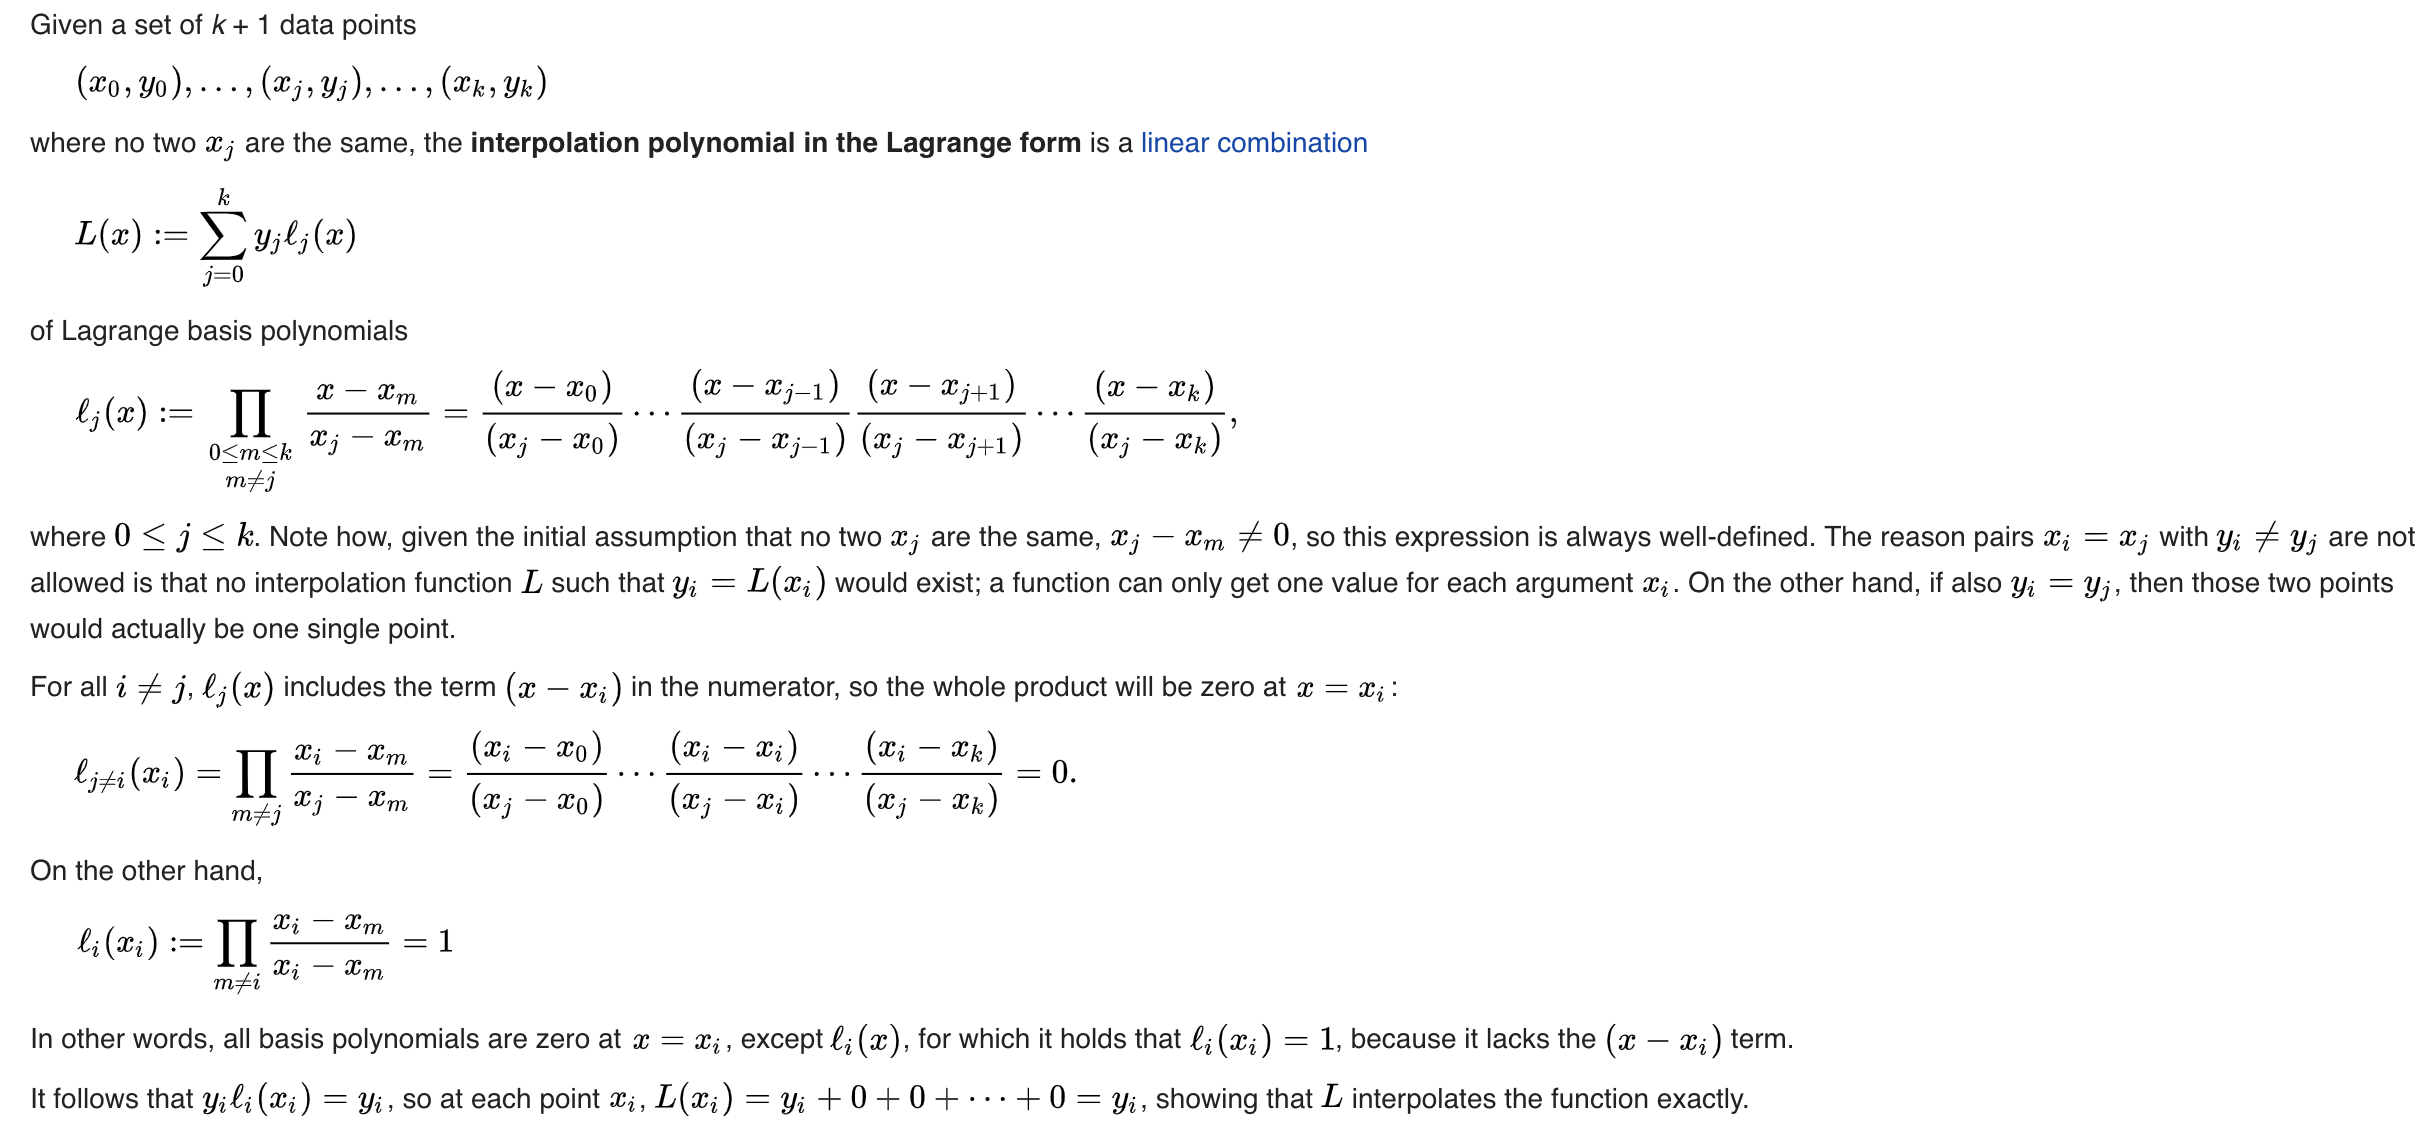
\includegraphics{Lagrange_def.png}
\caption{title}
\end{figure}

    \begin{Verbatim}[commandchars=\\\{\}]
{\color{incolor}In [{\color{incolor}3}]:} \PY{k}{using} \PY{n}{Polynomials}
        \PY{k}{using} \PY{n}{Plots}
\end{Verbatim}


    \begin{Verbatim}[commandchars=\\\{\}]
{\color{incolor}In [{\color{incolor}4}]:} \PY{k}{function} \PY{n}{l}\PY{p}{(}\PY{n}{k}\PY{p}{,} \PY{n}{X}\PY{p}{)}
            \PY{n}{x\PYZus{}k} \PY{o}{=} \PY{n}{X}\PY{p}{[}\PY{n}{k}\PY{p}{]}
            \PY{n}{X} \PY{o}{=} \PY{p}{[}\PY{n}{x} \PY{k}{for} \PY{n}{x} \PY{k+kp}{in} \PY{n}{X} \PY{k}{if} \PY{n}{x} \PY{o}{!=} \PY{n}{x\PYZus{}k}\PY{p}{]}
            \PY{n}{p} \PY{o}{=} \PY{n}{Poly}\PY{p}{(}\PY{p}{[}\PY{l+m+mf}{1.0}\PY{p}{]}\PY{p}{)}
            \PY{n}{q} \PY{o}{=} \PY{l+m+mi}{1}
            \PY{k}{for} \PY{n}{x\PYZus{}i} \PY{k+kp}{in} \PY{n}{X}
                \PY{n}{p} \PY{o}{=} \PY{n}{p} \PY{o}{*} \PY{n}{poly}\PY{p}{(}\PY{p}{[}\PY{n}{x\PYZus{}i}\PY{p}{]}\PY{p}{)}
                \PY{n}{q} \PY{o}{=} \PY{n}{q} \PY{o}{*} \PY{p}{(}\PY{n}{x\PYZus{}k} \PY{o}{\PYZhy{}} \PY{n}{x\PYZus{}i}\PY{p}{)}
            \PY{k}{end}
            \PY{k}{return} \PY{p}{(}\PY{n}{p} \PY{o}{/} \PY{n}{q}\PY{p}{)}
        \PY{k}{end}
        
        \PY{k}{function} \PY{n}{L}\PY{p}{(}\PY{n}{X}\PY{p}{,} \PY{n}{Y}\PY{p}{)}
            \PY{n}{p} \PY{o}{=} \PY{n}{Poly}\PY{p}{(}\PY{p}{[}\PY{l+m+mi}{0}\PY{p}{]}\PY{p}{)}
            \PY{k}{for} \PY{n}{k} \PY{k+kp}{in} \PY{l+m+mi}{1}\PY{o}{:}\PY{l+m+mi}{1}\PY{o}{:}\PY{n}{length}\PY{p}{(}\PY{n}{Y}\PY{p}{)}
                \PY{n}{p} \PY{o}{=} \PY{n}{p} \PY{o}{+} \PY{p}{(}\PY{n}{Y}\PY{p}{[}\PY{n}{k}\PY{p}{]} \PY{o}{*} \PY{n}{l}\PY{p}{(}\PY{n}{k}\PY{p}{,} \PY{n}{X}\PY{p}{)}\PY{p}{)}
            \PY{k}{end}
            \PY{k}{return} \PY{n}{p}
        \PY{k}{end}
\end{Verbatim}


\begin{Verbatim}[commandchars=\\\{\}]
{\color{outcolor}Out[{\color{outcolor}4}]:} L (generic function with 1 method)
\end{Verbatim}
            
    \begin{Verbatim}[commandchars=\\\{\}]
{\color{incolor}In [{\color{incolor}43}]:} \PY{n}{x} \PY{o}{=} \PY{l+m+mi}{1}\PY{o}{:}\PY{l+m+mi}{1}\PY{o}{:}\PY{l+m+mi}{10}
         \PY{n}{y} \PY{o}{=} \PY{p}{[}\PY{n}{rand}\PY{p}{(}\PY{p}{)} \PY{k}{for} \PY{n}{a} \PY{k+kp}{in} \PY{n}{x}\PY{p}{]}
         \PY{n}{xs} \PY{o}{=} \PY{l+m+mf}{1.0}\PY{o}{:}\PY{l+m+mf}{0.05}\PY{o}{:}\PY{l+m+mf}{10.0}
\end{Verbatim}


\begin{Verbatim}[commandchars=\\\{\}]
{\color{outcolor}Out[{\color{outcolor}43}]:} 1.0:0.05:10.0
\end{Verbatim}
            
    \begin{Verbatim}[commandchars=\\\{\}]
{\color{incolor}In [{\color{incolor}44}]:} \PY{n}{equL} \PY{o}{=} \PY{n}{L}\PY{p}{(}\PY{n}{x}\PY{p}{,} \PY{n}{y}\PY{p}{)}
         
         \PY{n}{scatter}\PY{p}{(}\PY{n}{x}\PY{p}{,} \PY{n}{y}\PY{p}{,} \PY{n}{label} \PY{o}{=} \PY{l+s}{\PYZdq{}}\PY{l+s}{d}\PY{l+s}{a}\PY{l+s}{t}\PY{l+s}{a}\PY{l+s}{ }\PY{l+s}{p}\PY{l+s}{o}\PY{l+s}{i}\PY{l+s}{n}\PY{l+s}{t}\PY{l+s}{s}\PY{l+s}{\PYZdq{}}\PY{p}{)}
         
         \PY{n}{plot!}\PY{p}{(}\PY{n}{xs}\PY{p}{,} \PY{n}{polyval}\PY{p}{(}\PY{n}{equL}\PY{p}{,} \PY{n}{xs}\PY{p}{)}\PY{p}{,}
             \PY{n}{color}\PY{o}{=}\PY{o}{:}\PY{n}{pink}\PY{p}{,}
             \PY{n}{label} \PY{o}{=} \PY{l+s}{\PYZdq{}}\PY{l+s}{L}\PY{l+s}{a}\PY{l+s}{g}\PY{l+s}{r}\PY{l+s}{a}\PY{l+s}{n}\PY{l+s}{g}\PY{l+s}{e}\PY{l+s}{ }\PY{l+s}{i}\PY{l+s}{n}\PY{l+s}{t}\PY{l+s}{e}\PY{l+s}{r}\PY{l+s}{p}\PY{l+s}{o}\PY{l+s}{l}\PY{l+s}{a}\PY{l+s}{t}\PY{l+s}{i}\PY{l+s}{o}\PY{l+s}{n}\PY{l+s}{\PYZdq{}}\PY{p}{,}
             \PY{n}{xlabel} \PY{o}{=} \PY{l+s}{\PYZdq{}}\PY{l+s}{X}\PY{l+s}{\PYZdq{}}\PY{p}{,}
             \PY{n}{ylabel} \PY{o}{=} \PY{l+s}{\PYZdq{}}\PY{l+s}{Y}\PY{l+s}{\PYZdq{}}\PY{p}{,}
             \PY{n}{title} \PY{o}{=} \PY{l+s}{\PYZdq{}}\PY{l+s}{L}\PY{l+s}{a}\PY{l+s}{g}\PY{l+s}{r}\PY{l+s}{a}\PY{l+s}{n}\PY{l+s}{g}\PY{l+s}{e}\PY{l+s}{ }\PY{l+s}{i}\PY{l+s}{n}\PY{l+s}{t}\PY{l+s}{e}\PY{l+s}{r}\PY{l+s}{p}\PY{l+s}{o}\PY{l+s}{l}\PY{l+s}{a}\PY{l+s}{t}\PY{l+s}{i}\PY{l+s}{o}\PY{l+s}{n}\PY{l+s}{\PYZdq{}}\PY{p}{,}
             \PY{n}{dpi} \PY{o}{=} \PY{l+m+mi}{120}\PY{p}{,}
             \PY{n}{size} \PY{o}{=} \PY{p}{(}\PY{l+m+mi}{600}\PY{p}{,}\PY{l+m+mi}{500}\PY{p}{)}
             \PY{p}{)}
\end{Verbatim}

\texttt{\color{outcolor}Out[{\color{outcolor}44}]:}
    
    \begin{center}
    \adjustimage{max size={0.9\linewidth}{0.9\paperheight}}{output_7_0.pdf}
    \end{center}
    { \hspace*{\fill} \\}
    

    \hypertarget{newton}{%
\subsection{Newton}\label{newton}}

    Zrobic to samo dla metody Newtona (metoda ilorazów róznicowych). Zadbac
o to, żeby ilorazy wyliczać tylko raz dla danego zbioru wezłow
interpolacji. Jezyk implementacji wybrac taki sam, jak w poprzednim
punkcie. Narysować wykres wielomianu interpolacyjnego dla tych samych
danych, co w poprzednim punkcie.

    \begin{figure}
\centering
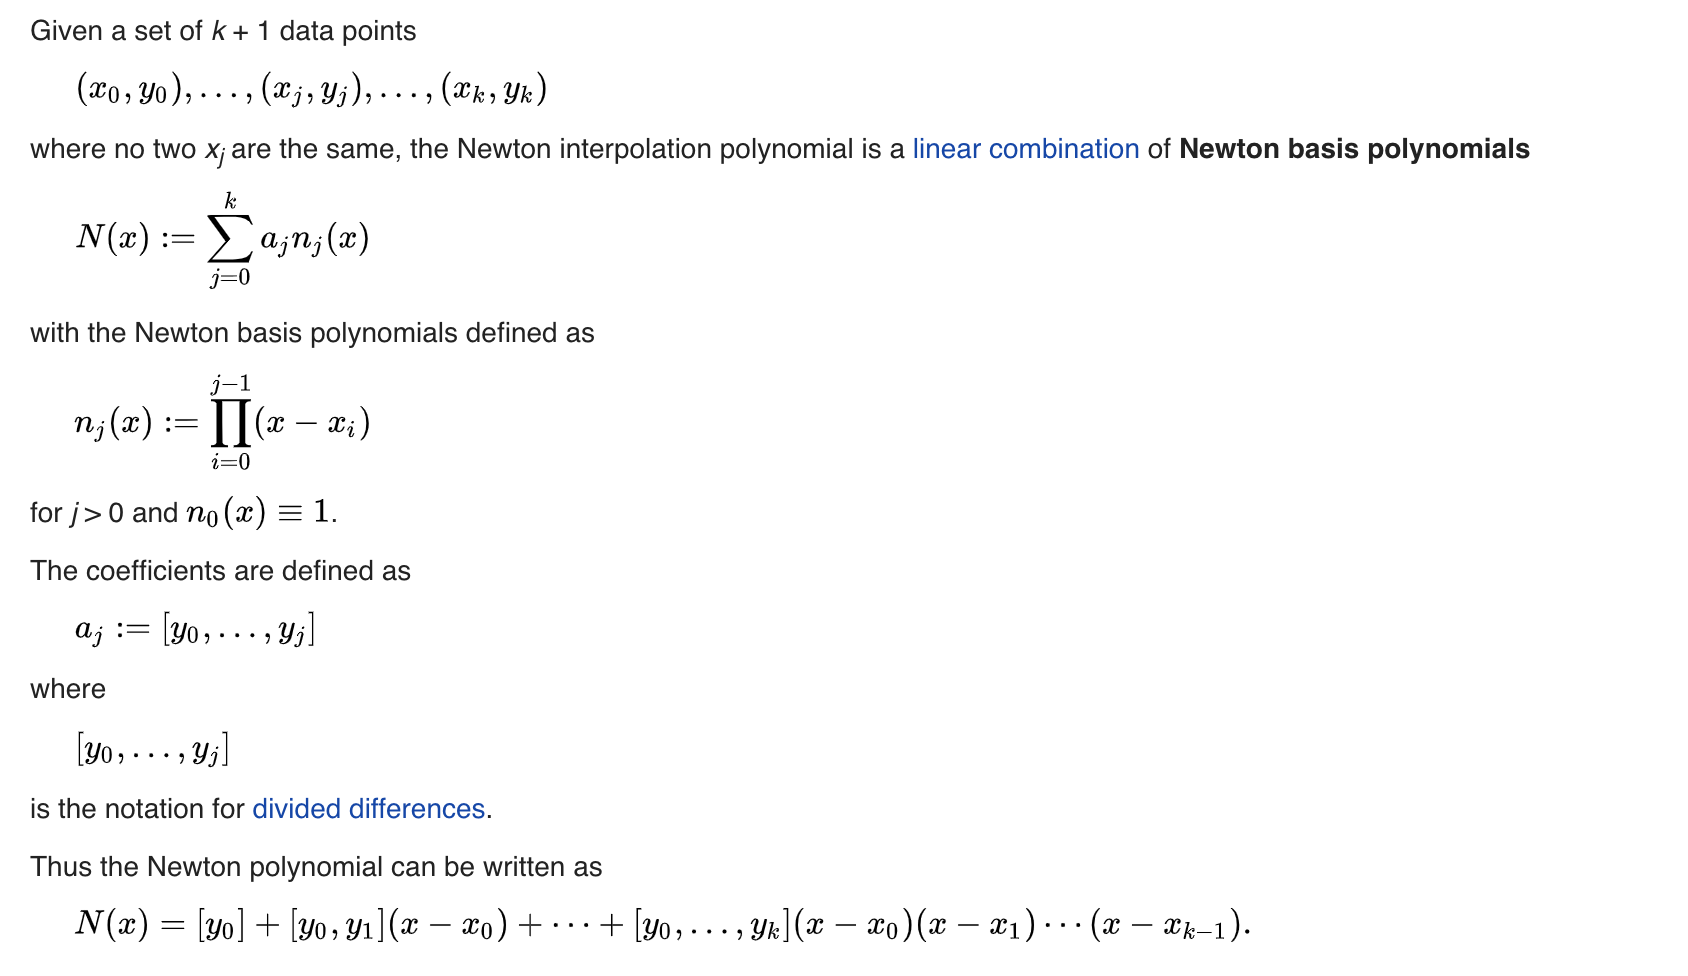
\includegraphics{Newton_def.png}
\caption{title}
\end{figure}

    \begin{Verbatim}[commandchars=\\\{\}]
{\color{incolor}In [{\color{incolor}20}]:} \PY{k}{function} \PY{n}{comp\PYZus{}n}\PY{p}{(}\PY{n}{X}\PY{p}{,} \PY{n}{y\PYZus{}k}\PY{p}{,} \PY{n}{k}\PY{p}{,} \PY{n}{p\PYZus{}k}\PY{p}{)}
             \PY{n}{x\PYZus{}k} \PY{o}{=} \PY{n}{X}\PY{p}{[}\PY{n}{k}\PY{p}{]}
             \PY{n}{p} \PY{o}{=} \PY{n}{y\PYZus{}k} \PY{o}{\PYZhy{}} \PY{n}{polyval}\PY{p}{(}\PY{n}{p\PYZus{}k}\PY{p}{,} \PY{n}{x\PYZus{}k}\PY{p}{)}
             \PY{n}{q} \PY{o}{=} \PY{l+m+mi}{1}
             \PY{k}{for} \PY{n}{i} \PY{k+kp}{in} \PY{l+m+mi}{1}\PY{o}{:}\PY{l+m+mi}{1}\PY{o}{:}\PY{n}{k}\PY{o}{\PYZhy{}}\PY{l+m+mi}{1}
                 \PY{n}{q} \PY{o}{=} \PY{n}{q} \PY{o}{*} \PY{p}{(}\PY{n}{x\PYZus{}k} \PY{o}{\PYZhy{}} \PY{n}{X}\PY{p}{[}\PY{n}{i}\PY{p}{]}\PY{p}{)}
             \PY{k}{end}
             \PY{k}{return} \PY{p}{(}\PY{n}{p} \PY{o}{/} \PY{n}{q}\PY{p}{)}
         \PY{k}{end}
         
         \PY{k}{function} \PY{n}{N}\PY{p}{(}\PY{n}{X}\PY{p}{,} \PY{n}{Y}\PY{p}{,} \PY{n}{n}\PY{p}{)}
             \PY{k}{if} \PY{n}{n} \PY{o}{==} \PY{l+m+mi}{1}
                 \PY{n}{Poly}\PY{p}{(}\PY{n}{float}\PY{p}{(}\PY{n}{Y}\PY{p}{[}\PY{l+m+mi}{1}\PY{p}{]}\PY{p}{)}\PY{p}{)}
             \PY{k}{else}
                 \PY{n}{pp} \PY{o}{=} \PY{n}{N}\PY{p}{(}\PY{n}{X}\PY{p}{,} \PY{n}{Y}\PY{p}{,} \PY{n}{n}\PY{o}{\PYZhy{}}\PY{l+m+mi}{1}\PY{p}{)}
                 \PY{n}{c} \PY{o}{=} \PY{n}{comp\PYZus{}n}\PY{p}{(}\PY{n}{X}\PY{p}{,} \PY{n}{Y}\PY{p}{[}\PY{n}{n}\PY{p}{]}\PY{p}{,} \PY{n}{n}\PY{p}{,} \PY{n}{pp}\PY{p}{)}
                 \PY{n}{poly}\PY{p}{(}\PY{p}{[}\PY{n}{X}\PY{p}{[}\PY{n}{i}\PY{p}{]} \PY{k}{for} \PY{n}{i} \PY{k+kp}{in} \PY{l+m+mi}{1}\PY{o}{:}\PY{l+m+mi}{1}\PY{o}{:}\PY{n}{n}\PY{o}{\PYZhy{}}\PY{l+m+mi}{1}\PY{p}{]}\PY{p}{)} \PY{o}{*} \PY{n}{c} \PY{o}{+} \PY{n}{pp}
             \PY{k}{end}
         \PY{k}{end}
         
         \PY{k}{function} \PY{n}{N}\PY{p}{(}\PY{n}{X}\PY{p}{,} \PY{n}{Y}\PY{p}{)}
             \PY{n}{N}\PY{p}{(}\PY{n}{X}\PY{p}{,} \PY{n}{Y}\PY{p}{,} \PY{n}{length}\PY{p}{(}\PY{n}{Y}\PY{p}{)}\PY{p}{)}
         \PY{k}{end}
\end{Verbatim}


\begin{Verbatim}[commandchars=\\\{\}]
{\color{outcolor}Out[{\color{outcolor}20}]:} N (generic function with 2 methods)
\end{Verbatim}
            
    \begin{Verbatim}[commandchars=\\\{\}]
{\color{incolor}In [{\color{incolor}45}]:} \PY{n}{equN} \PY{o}{=} \PY{n}{N}\PY{p}{(}\PY{n}{x}\PY{p}{,} \PY{n}{y}\PY{p}{)}
         
         \PY{n}{scatter}\PY{p}{(}\PY{n}{x}\PY{p}{,} \PY{n}{y}\PY{p}{,}\PY{n}{label} \PY{o}{=} \PY{l+s}{\PYZdq{}}\PY{l+s}{d}\PY{l+s}{a}\PY{l+s}{t}\PY{l+s}{a}\PY{l+s}{ }\PY{l+s}{p}\PY{l+s}{o}\PY{l+s}{i}\PY{l+s}{n}\PY{l+s}{t}\PY{l+s}{s}\PY{l+s}{\PYZdq{}}\PY{p}{)}
         
         \PY{n}{plot!}\PY{p}{(}\PY{n}{xs}\PY{p}{,} \PY{n}{polyval}\PY{p}{(}\PY{n}{equN}\PY{p}{,} \PY{n}{xs}\PY{p}{)}\PY{p}{,}
             \PY{n}{color}\PY{o}{=}\PY{o}{:}\PY{n}{brown}\PY{p}{,}
             \PY{n}{label} \PY{o}{=} \PY{l+s}{\PYZdq{}}\PY{l+s}{N}\PY{l+s}{e}\PY{l+s}{w}\PY{l+s}{t}\PY{l+s}{o}\PY{l+s}{n}\PY{l+s}{ }\PY{l+s}{i}\PY{l+s}{n}\PY{l+s}{t}\PY{l+s}{e}\PY{l+s}{r}\PY{l+s}{p}\PY{l+s}{o}\PY{l+s}{l}\PY{l+s}{a}\PY{l+s}{t}\PY{l+s}{i}\PY{l+s}{o}\PY{l+s}{n}\PY{l+s}{\PYZdq{}}\PY{p}{,}
             \PY{n}{xlabel} \PY{o}{=} \PY{l+s}{\PYZdq{}}\PY{l+s}{X}\PY{l+s}{\PYZdq{}}\PY{p}{,}
             \PY{n}{ylabel} \PY{o}{=} \PY{l+s}{\PYZdq{}}\PY{l+s}{Y}\PY{l+s}{\PYZdq{}}\PY{p}{,}
             \PY{n}{title} \PY{o}{=} \PY{l+s}{\PYZdq{}}\PY{l+s}{N}\PY{l+s}{e}\PY{l+s}{w}\PY{l+s}{t}\PY{l+s}{o}\PY{l+s}{n}\PY{l+s}{ }\PY{l+s}{i}\PY{l+s}{n}\PY{l+s}{t}\PY{l+s}{e}\PY{l+s}{r}\PY{l+s}{p}\PY{l+s}{o}\PY{l+s}{l}\PY{l+s}{a}\PY{l+s}{t}\PY{l+s}{i}\PY{l+s}{o}\PY{l+s}{n}\PY{l+s}{\PYZdq{}}\PY{p}{,}
             \PY{n}{dpi} \PY{o}{=} \PY{l+m+mi}{120}\PY{p}{,}
             \PY{n}{size} \PY{o}{=} \PY{p}{(}\PY{l+m+mi}{600}\PY{p}{,}\PY{l+m+mi}{500}\PY{p}{)}\PY{p}{)}
\end{Verbatim}

\texttt{\color{outcolor}Out[{\color{outcolor}45}]:}
    
    \begin{center}
    \adjustimage{max size={0.9\linewidth}{0.9\paperheight}}{output_12_0.pdf}
    \end{center}
    { \hspace*{\fill} \\}
    

    \hypertarget{polynomials}{%
\subsection{Polynomials}\label{polynomials}}

    Zastosowac interpolację wielomianową z pakietu Polynomials do tych
samych danych, co w poprzednich punktach. Porównać wszystkie 3 wyniki
interpolacji wielomianowej na jednym wykresie. Co zauważamy? Dlaczego?

    \begin{Verbatim}[commandchars=\\\{\}]
{\color{incolor}In [{\color{incolor}46}]:} \PY{n}{equP} \PY{o}{=} \PY{n}{polyfit}\PY{p}{(}\PY{n}{x}\PY{p}{,} \PY{n}{y}\PY{p}{)}
         
         \PY{n}{scatter}\PY{p}{(}\PY{n}{x}\PY{p}{,} \PY{n}{y}\PY{p}{,} \PY{n}{label} \PY{o}{=} \PY{l+s}{\PYZdq{}}\PY{l+s}{d}\PY{l+s}{a}\PY{l+s}{t}\PY{l+s}{a}\PY{l+s}{ }\PY{l+s}{p}\PY{l+s}{o}\PY{l+s}{i}\PY{l+s}{n}\PY{l+s}{t}\PY{l+s}{s}\PY{l+s}{\PYZdq{}}\PY{p}{)}
         
         \PY{n}{plot!}\PY{p}{(}\PY{n}{xs}\PY{p}{,} \PY{n}{polyval}\PY{p}{(}\PY{n}{equL}\PY{p}{,} \PY{n}{xs}\PY{p}{)}\PY{p}{,}
             \PY{n}{color}\PY{o}{=}\PY{o}{:}\PY{n}{pink}\PY{p}{,}
             \PY{n}{label} \PY{o}{=} \PY{l+s}{\PYZdq{}}\PY{l+s}{L}\PY{l+s}{a}\PY{l+s}{g}\PY{l+s}{r}\PY{l+s}{a}\PY{l+s}{n}\PY{l+s}{g}\PY{l+s}{e}\PY{l+s}{ }\PY{l+s}{i}\PY{l+s}{n}\PY{l+s}{t}\PY{l+s}{e}\PY{l+s}{r}\PY{l+s}{p}\PY{l+s}{o}\PY{l+s}{l}\PY{l+s}{a}\PY{l+s}{t}\PY{l+s}{i}\PY{l+s}{o}\PY{l+s}{n}\PY{l+s}{\PYZdq{}}\PY{p}{,}
         \PY{p}{)}
         
         \PY{n}{plot!}\PY{p}{(}\PY{n}{xs}\PY{p}{,} \PY{n}{polyval}\PY{p}{(}\PY{n}{equN}\PY{p}{,} \PY{n}{xs}\PY{p}{)}\PY{p}{,}
             \PY{n}{color}\PY{o}{=}\PY{o}{:}\PY{n}{brown}\PY{p}{,}
             \PY{n}{label} \PY{o}{=} \PY{l+s}{\PYZdq{}}\PY{l+s}{N}\PY{l+s}{e}\PY{l+s}{w}\PY{l+s}{t}\PY{l+s}{o}\PY{l+s}{n}\PY{l+s}{ }\PY{l+s}{i}\PY{l+s}{n}\PY{l+s}{t}\PY{l+s}{e}\PY{l+s}{r}\PY{l+s}{p}\PY{l+s}{o}\PY{l+s}{l}\PY{l+s}{a}\PY{l+s}{t}\PY{l+s}{i}\PY{l+s}{o}\PY{l+s}{n}\PY{l+s}{\PYZdq{}}\PY{p}{)}
         
         \PY{n}{plot!}\PY{p}{(}\PY{n}{xs}\PY{p}{,} \PY{n}{polyval}\PY{p}{(}\PY{n}{equP}\PY{p}{,} \PY{n}{xs}\PY{p}{)}\PY{p}{,}
             \PY{n}{color}\PY{o}{=}\PY{o}{:}\PY{n}{red}\PY{p}{,}
             \PY{n}{label} \PY{o}{=} \PY{l+s}{\PYZdq{}}\PY{l+s}{P}\PY{l+s}{o}\PY{l+s}{l}\PY{l+s}{y}\PY{l+s}{n}\PY{l+s}{o}\PY{l+s}{m}\PY{l+s}{i}\PY{l+s}{a}\PY{l+s}{l}\PY{l+s}{\PYZhy{}}\PY{l+s}{p}\PY{l+s}{o}\PY{l+s}{l}\PY{l+s}{y}\PY{l+s}{f}\PY{l+s}{i}\PY{l+s}{t}\PY{l+s}{ }\PY{l+s}{i}\PY{l+s}{n}\PY{l+s}{t}\PY{l+s}{e}\PY{l+s}{r}\PY{l+s}{p}\PY{l+s}{o}\PY{l+s}{l}\PY{l+s}{a}\PY{l+s}{t}\PY{l+s}{i}\PY{l+s}{o}\PY{l+s}{n}\PY{l+s}{\PYZdq{}}\PY{p}{,}
             \PY{n}{xlabel} \PY{o}{=} \PY{l+s}{\PYZdq{}}\PY{l+s}{X}\PY{l+s}{\PYZdq{}}\PY{p}{,}
             \PY{n}{ylabel} \PY{o}{=} \PY{l+s}{\PYZdq{}}\PY{l+s}{Y}\PY{l+s}{\PYZdq{}}\PY{p}{,}
             \PY{n}{title} \PY{o}{=} \PY{l+s}{\PYZdq{}}\PY{l+s}{N}\PY{l+s}{e}\PY{l+s}{w}\PY{l+s}{t}\PY{l+s}{o}\PY{l+s}{n}\PY{l+s}{,}\PY{l+s}{ }\PY{l+s}{L}\PY{l+s}{a}\PY{l+s}{g}\PY{l+s}{r}\PY{l+s}{a}\PY{l+s}{n}\PY{l+s}{g}\PY{l+s}{e}\PY{l+s}{,}\PY{l+s}{ }\PY{l+s}{P}\PY{l+s}{o}\PY{l+s}{l}\PY{l+s}{y}\PY{l+s}{n}\PY{l+s}{o}\PY{l+s}{m}\PY{l+s}{i}\PY{l+s}{a}\PY{l+s}{l}\PY{l+s}{ }\PY{l+s}{i}\PY{l+s}{n}\PY{l+s}{t}\PY{l+s}{e}\PY{l+s}{r}\PY{l+s}{p}\PY{l+s}{o}\PY{l+s}{l}\PY{l+s}{a}\PY{l+s}{t}\PY{l+s}{i}\PY{l+s}{o}\PY{l+s}{n}\PY{l+s}{\PYZdq{}}\PY{p}{,}
             \PY{n}{dpi} \PY{o}{=} \PY{l+m+mi}{120}\PY{p}{,}
             \PY{n}{size} \PY{o}{=} \PY{p}{(}\PY{l+m+mi}{600}\PY{p}{,}\PY{l+m+mi}{500}\PY{p}{)}\PY{p}{)}
\end{Verbatim}

\texttt{\color{outcolor}Out[{\color{outcolor}46}]:}
    
    \begin{center}
    \adjustimage{max size={0.9\linewidth}{0.9\paperheight}}{output_15_0.pdf}
    \end{center}
    { \hspace*{\fill} \\}
    

    Każdy z interpolujących wielomianów prechodzi przez te same punkty.
Dzieje się tak, gdyż dla danych n+1 punktów istnieje dokładnie jeden
wielomian n-tego stopnia, który przez nie przechodzi.

    \hypertarget{analiza}{%
\subsection{Analiza}\label{analiza}}

    Porownać metody poprzez pomiar czasu wykonania dla zmiennej ilości
węzłow interpolacji. Dokonac pomiaru 10 razy i policzyc wartość średnią
oraz oszacować bład pomiaru za pomoca odchylenia standardowego.

    \begin{Verbatim}[commandchars=\\\{\}]
{\color{incolor}In [{\color{incolor}26}]:} \PY{k}{using} \PY{n}{DataFrames}
         \PY{k}{using} \PY{n}{Statistics}
\end{Verbatim}


    \begin{Verbatim}[commandchars=\\\{\}]
{\color{incolor}In [{\color{incolor}50}]:} \PY{n}{df} \PY{o}{=} \PY{n}{DataFrame}\PY{p}{(}\PY{k}{type}\PY{o}{=}\PY{n}{String}\PY{p}{[}\PY{p}{]}\PY{p}{,} \PY{n}{size} \PY{o}{=} \PY{k+kt}{Int64}\PY{p}{[}\PY{p}{]}\PY{p}{,} \PY{n}{time} \PY{o}{=} \PY{k+kt}{Float64}\PY{p}{[}\PY{p}{]}\PY{p}{)}
                 
         \PY{n}{types}\PY{o}{=}\PY{p}{[}\PY{p}{]}\PY{p}{;}\PY{n}{sizes}\PY{o}{=}\PY{p}{[}\PY{p}{]}\PY{p}{;}\PY{n}{times}\PY{o}{=}\PY{p}{[}\PY{p}{]}
         \PY{n}{range} \PY{o}{=} \PY{l+m+mi}{100}\PY{o}{:}\PY{l+m+mi}{100}\PY{o}{:}\PY{l+m+mi}{500}
         \PY{k}{for} \PY{n}{rr} \PY{k+kp}{in} \PY{n}{range}
             \PY{n}{xx} \PY{o}{=} \PY{l+m+mi}{0}\PY{o}{:}\PY{l+m+mi}{1}\PY{o}{:}\PY{n}{rr}
             \PY{k}{for} \PY{n}{i} \PY{k+kp}{in} \PY{l+m+mi}{1}\PY{o}{:}\PY{l+m+mi}{1}\PY{o}{:}\PY{l+m+mi}{10}
                 \PY{n}{yy} \PY{o}{=} \PY{n}{rand}\PY{p}{(}\PY{k+kt}{Int}\PY{p}{,} \PY{n}{rr}\PY{o}{+}\PY{l+m+mi}{1}\PY{p}{)}
                 \PY{n}{push!}\PY{p}{(}\PY{n}{df}\PY{p}{,}\PY{p}{[}\PY{l+s}{\PYZdq{}}\PY{l+s}{l}\PY{l+s}{a}\PY{l+s}{g}\PY{l+s}{r}\PY{l+s}{a}\PY{l+s}{n}\PY{l+s}{g}\PY{l+s}{e}\PY{l+s}{\PYZdq{}}\PY{p}{,} \PY{n}{rr}\PY{p}{,} \PY{n+nd}{@elapsed} \PY{n}{L}\PY{p}{(}\PY{n}{xx}\PY{p}{,}\PY{n}{yy}\PY{p}{)}\PY{p}{]}\PY{p}{)}        
                 \PY{n}{push!}\PY{p}{(}\PY{n}{df}\PY{p}{,} \PY{p}{[}\PY{l+s}{\PYZdq{}}\PY{l+s}{n}\PY{l+s}{e}\PY{l+s}{w}\PY{l+s}{t}\PY{l+s}{o}\PY{l+s}{n}\PY{l+s}{\PYZdq{}}\PY{p}{,} \PY{n}{rr}\PY{p}{,} \PY{n+nd}{@elapsed} \PY{n}{N}\PY{p}{(}\PY{n}{xx}\PY{p}{,}\PY{n}{yy}\PY{p}{)}\PY{p}{]}\PY{p}{)}
                 \PY{n}{push!}\PY{p}{(}\PY{n}{df}\PY{p}{,} \PY{p}{[}\PY{l+s}{\PYZdq{}}\PY{l+s}{p}\PY{l+s}{o}\PY{l+s}{l}\PY{l+s}{y}\PY{l+s}{f}\PY{l+s}{i}\PY{l+s}{t}\PY{l+s}{\PYZdq{}}\PY{p}{,} \PY{n}{rr}\PY{p}{,} \PY{n+nd}{@elapsed} \PY{n}{polyfit}\PY{p}{(}\PY{n}{xx}\PY{p}{,}\PY{n}{yy}\PY{p}{)}\PY{p}{]}\PY{p}{)}
             \PY{k}{end}
         \PY{k}{end}
         \PY{n}{df}
\end{Verbatim}


\begin{Verbatim}[commandchars=\\\{\}]
{\color{outcolor}Out[{\color{outcolor}50}]:} 150×3 DataFrame
         │ Row │ type     │ size  │ time        │
         │     │ String   │ Int64 │ Float64     │
         ├─────┼──────────┼───────┼─────────────┤
         │ 1   │ lagrange │ 100   │ 0.0156968   │
         │ 2   │ newton   │ 100   │ 0.00058451  │
         │ 3   │ polyfit  │ 100   │ 0.000611382 │
         │ 4   │ lagrange │ 100   │ 0.0173896   │
         │ 5   │ newton   │ 100   │ 0.000501716 │
         │ 6   │ polyfit  │ 100   │ 0.000198969 │
         │ 7   │ lagrange │ 100   │ 0.00677467  │
         │ 8   │ newton   │ 100   │ 0.000429562 │
         │ 9   │ polyfit  │ 100   │ 0.000170501 │
         │ 10  │ lagrange │ 100   │ 0.0112772   │
         ⋮
         │ 140 │ newton   │ 500   │ 0.0194804   │
         │ 141 │ polyfit  │ 500   │ 0.00374528  │
         │ 142 │ lagrange │ 500   │ 0.544991    │
         │ 143 │ newton   │ 500   │ 0.0227626   │
         │ 144 │ polyfit  │ 500   │ 0.00375438  │
         │ 145 │ lagrange │ 500   │ 0.551041    │
         │ 146 │ newton   │ 500   │ 0.0194777   │
         │ 147 │ polyfit  │ 500   │ 0.0038756   │
         │ 148 │ lagrange │ 500   │ 0.549014    │
         │ 149 │ newton   │ 500   │ 0.0195353   │
         │ 150 │ polyfit  │ 500   │ 0.00622336  │
\end{Verbatim}
            
    \begin{Verbatim}[commandchars=\\\{\}]
{\color{incolor}In [{\color{incolor}51}]:} \PY{n}{pol\PYZus{}res} \PY{o}{=} \PY{n}{by}\PY{p}{(}\PY{n}{df}\PY{p}{,} \PY{p}{[}\PY{l+m+mi}{1}\PY{p}{,}\PY{l+m+mi}{2}\PY{p}{]}\PY{p}{)} \PY{k}{do} \PY{n}{dff}
             \PY{n}{DataFrame}\PY{p}{(}\PY{n}{time\PYZus{}mean} \PY{o}{=} \PY{n}{mean}\PY{p}{(}\PY{n}{dff}\PY{p}{[}\PY{l+m+mi}{3}\PY{p}{]}\PY{p}{)}\PY{p}{,} \PY{n}{time\PYZus{}std} \PY{o}{=} \PY{n}{std}\PY{p}{(}\PY{n}{dff}\PY{p}{[}\PY{l+m+mi}{3}\PY{p}{]}\PY{p}{)}\PY{p}{)}
         \PY{k}{end}
\end{Verbatim}


\begin{Verbatim}[commandchars=\\\{\}]
{\color{outcolor}Out[{\color{outcolor}51}]:} 15×4 DataFrame
         │ Row │ type     │ size  │ time\_mean   │ time\_std    │
         │     │ String   │ Int64 │ Float64     │ Float64     │
         ├─────┼──────────┼───────┼─────────────┼─────────────┤
         │ 1   │ lagrange │ 100   │ 0.0100212   │ 0.00435218  │
         │ 2   │ newton   │ 100   │ 0.000363283 │ 0.000105236 │
         │ 3   │ polyfit  │ 100   │ 0.000195765 │ 0.000147574 │
         │ 4   │ lagrange │ 200   │ 0.0405791   │ 0.00540252  │
         │ 5   │ newton   │ 200   │ 0.00191023  │ 0.000790464 │
         │ 6   │ polyfit  │ 200   │ 0.000724788 │ 0.000814945 │
         │ 7   │ lagrange │ 300   │ 0.127135    │ 0.00505647  │
         │ 8   │ newton   │ 300   │ 0.00477466  │ 0.000192925 │
         │ 9   │ polyfit  │ 300   │ 0.00120259  │ 0.000118685 │
         │ 10  │ lagrange │ 400   │ 0.28814     │ 0.0039224   │
         │ 11  │ newton   │ 400   │ 0.0118855   │ 0.00200529  │
         │ 12  │ polyfit  │ 400   │ 0.00283653  │ 0.00120733  │
         │ 13  │ lagrange │ 500   │ 0.54594     │ 0.0095752   │
         │ 14  │ newton   │ 500   │ 0.0206329   │ 0.00141171  │
         │ 15  │ polyfit  │ 500   │ 0.00458597  │ 0.00128937  │
\end{Verbatim}
            
    \begin{Verbatim}[commandchars=\\\{\}]
{\color{incolor}In [{\color{incolor}52}]:} \PY{n}{scatter}\PY{p}{(}\PY{n}{pol\PYZus{}res}\PY{p}{[}\PY{o}{:}\PY{n}{size}\PY{p}{]}\PY{p}{,} 
                 \PY{n}{pol\PYZus{}res}\PY{p}{[}\PY{o}{:}\PY{n}{time\PYZus{}mean}\PY{p}{]}\PY{p}{,} 
                 \PY{n}{group} \PY{o}{=} \PY{n}{pol\PYZus{}res}\PY{p}{[}\PY{o}{:}\PY{k}{type}\PY{p}{]}\PY{p}{,}
                 \PY{n}{yerr} \PY{o}{=} \PY{n}{pol\PYZus{}res}\PY{p}{[}\PY{o}{:}\PY{n}{time\PYZus{}std}\PY{p}{]}\PY{p}{,}
                 \PY{n}{xlabel} \PY{o}{=} \PY{l+s}{\PYZdq{}}\PY{l+s}{s}\PY{l+s}{i}\PY{l+s}{z}\PY{l+s}{e}\PY{l+s}{\PYZdq{}}\PY{p}{,}
                 \PY{n}{ylabel} \PY{o}{=} \PY{l+s}{\PYZdq{}}\PY{l+s}{t}\PY{l+s}{i}\PY{l+s}{m}\PY{l+s}{e}\PY{l+s}{ }\PY{l+s}{[}\PY{l+s}{s}\PY{l+s}{]}\PY{l+s}{\PYZdq{}}\PY{p}{,}
                 \PY{n}{dpi} \PY{o}{=} \PY{l+m+mi}{120}\PY{p}{,}
                 \PY{n}{size} \PY{o}{=} \PY{p}{(}\PY{l+m+mi}{600}\PY{p}{,}\PY{l+m+mi}{500}\PY{p}{)}\PY{p}{,}
                 \PY{n}{title} \PY{o}{=} \PY{l+s}{\PYZdq{}}\PY{l+s}{C}\PY{l+s}{o}\PY{l+s}{m}\PY{l+s}{p}\PY{l+s}{a}\PY{l+s}{r}\PY{l+s}{i}\PY{l+s}{s}\PY{l+s}{o}\PY{l+s}{n}\PY{l+s}{ }\PY{l+s}{o}\PY{l+s}{f}\PY{l+s}{ }\PY{l+s}{i}\PY{l+s}{n}\PY{l+s}{t}\PY{l+s}{e}\PY{l+s}{r}\PY{l+s}{p}\PY{l+s}{o}\PY{l+s}{l}\PY{l+s}{a}\PY{l+s}{t}\PY{l+s}{i}\PY{l+s}{o}\PY{l+s}{n}\PY{l+s}{ }\PY{l+s}{m}\PY{l+s}{e}\PY{l+s}{t}\PY{l+s}{h}\PY{l+s}{o}\PY{l+s}{d}\PY{l+s}{s}\PY{l+s}{\PYZdq{}}
                 \PY{p}{)}
\end{Verbatim}

\texttt{\color{outcolor}Out[{\color{outcolor}52}]:}
    
    \begin{center}
    \adjustimage{max size={0.9\linewidth}{0.9\paperheight}}{output_22_0.pdf}
    \end{center}
    { \hspace*{\fill} \\}
    

    \begin{Verbatim}[commandchars=\\\{\}]
{\color{incolor}In [{\color{incolor}53}]:} \PY{c}{\PYZsh{}\PYZsh{} dataframe without lagrange}
         \PY{n}{pol\PYZus{}res\PYZus{}noL} \PY{o}{=} \PY{n}{pol\PYZus{}res}\PY{p}{[}\PY{n}{pol\PYZus{}res}\PY{p}{[}\PY{o}{:}\PY{k}{type}\PY{p}{]}\PY{o}{.!=} \PY{l+s}{\PYZdq{}}\PY{l+s}{l}\PY{l+s}{a}\PY{l+s}{g}\PY{l+s}{r}\PY{l+s}{a}\PY{l+s}{n}\PY{l+s}{g}\PY{l+s}{e}\PY{l+s}{\PYZdq{}}\PY{p}{,} \PY{o}{:}\PY{p}{]}
         
         \PY{n}{scatter}\PY{p}{(}\PY{n}{pol\PYZus{}res\PYZus{}noL}\PY{p}{[}\PY{o}{:}\PY{n}{size}\PY{p}{]}\PY{p}{,} 
                 \PY{n}{pol\PYZus{}res\PYZus{}noL}\PY{p}{[}\PY{o}{:}\PY{n}{time\PYZus{}mean}\PY{p}{]}\PY{p}{,} 
                 \PY{n}{group} \PY{o}{=} \PY{n}{pol\PYZus{}res\PYZus{}noL}\PY{p}{[}\PY{o}{:}\PY{k}{type}\PY{p}{]}\PY{p}{,}
                 \PY{n}{yerr} \PY{o}{=} \PY{n}{pol\PYZus{}res\PYZus{}noL}\PY{p}{[}\PY{o}{:}\PY{n}{time\PYZus{}std}\PY{p}{]}\PY{p}{,}
                 \PY{n}{xlabel} \PY{o}{=} \PY{l+s}{\PYZdq{}}\PY{l+s}{s}\PY{l+s}{i}\PY{l+s}{z}\PY{l+s}{e}\PY{l+s}{\PYZdq{}}\PY{p}{,}
                 \PY{n}{ylabel} \PY{o}{=} \PY{l+s}{\PYZdq{}}\PY{l+s}{t}\PY{l+s}{i}\PY{l+s}{m}\PY{l+s}{e}\PY{l+s}{ }\PY{l+s}{[}\PY{l+s}{s}\PY{l+s}{]}\PY{l+s}{\PYZdq{}}\PY{p}{,}
                 \PY{n}{dpi} \PY{o}{=} \PY{l+m+mi}{120}\PY{p}{,}
                 \PY{n}{size} \PY{o}{=} \PY{p}{(}\PY{l+m+mi}{600}\PY{p}{,}\PY{l+m+mi}{500}\PY{p}{)}\PY{p}{,}
                 \PY{n}{title} \PY{o}{=} \PY{l+s}{\PYZdq{}}\PY{l+s}{C}\PY{l+s}{o}\PY{l+s}{m}\PY{l+s}{p}\PY{l+s}{a}\PY{l+s}{r}\PY{l+s}{i}\PY{l+s}{s}\PY{l+s}{o}\PY{l+s}{n}\PY{l+s}{ }\PY{l+s}{o}\PY{l+s}{f}\PY{l+s}{ }\PY{l+s}{i}\PY{l+s}{n}\PY{l+s}{t}\PY{l+s}{e}\PY{l+s}{r}\PY{l+s}{p}\PY{l+s}{o}\PY{l+s}{l}\PY{l+s}{a}\PY{l+s}{t}\PY{l+s}{i}\PY{l+s}{o}\PY{l+s}{n}\PY{l+s}{ }\PY{l+s}{m}\PY{l+s}{e}\PY{l+s}{t}\PY{l+s}{h}\PY{l+s}{o}\PY{l+s}{d}\PY{l+s}{s}\PY{l+s}{\PYZdq{}}\PY{p}{)}
\end{Verbatim}

\texttt{\color{outcolor}Out[{\color{outcolor}53}]:}
    
    \begin{center}
    \adjustimage{max size={0.9\linewidth}{0.9\paperheight}}{output_23_0.pdf}
    \end{center}
    { \hspace*{\fill} \\}
    

    \hypertarget{eksperyment}{%
\subsection{Eksperyment}\label{eksperyment}}

    Poeksperymentowac z interpolacją funkcjami sklejanymi (minimum dwie
rozne funkcje sklejane), narysowac wykresy i porownac z wykresami
interpolacji wielomianowej.

    \begin{Verbatim}[commandchars=\\\{\}]
{\color{incolor}In [{\color{incolor}37}]:} \PY{k}{using} \PY{n}{Interpolations}
\end{Verbatim}


    \begin{Verbatim}[commandchars=\\\{\}]
{\color{incolor}In [{\color{incolor}54}]:} \PY{n}{scatter}\PY{p}{(}\PY{n}{x}\PY{p}{,} \PY{n}{y}\PY{p}{,} \PY{n}{label} \PY{o}{=} \PY{l+s}{\PYZdq{}}\PY{l+s}{d}\PY{l+s}{a}\PY{l+s}{t}\PY{l+s}{a}\PY{l+s}{ }\PY{l+s}{p}\PY{l+s}{o}\PY{l+s}{i}\PY{l+s}{n}\PY{l+s}{t}\PY{l+s}{s}\PY{l+s}{\PYZdq{}}\PY{p}{)}
         
          \PY{n}{plot!}\PY{p}{(}\PY{n}{xs}\PY{p}{,} \PY{n}{polyval}\PY{p}{(}\PY{n}{equL}\PY{p}{,} \PY{n}{xs}\PY{p}{)}\PY{p}{,}
              \PY{n}{color}\PY{o}{=}\PY{o}{:}\PY{n}{pink}\PY{p}{,}
              \PY{n}{label} \PY{o}{=} \PY{l+s}{\PYZdq{}}\PY{l+s}{L}\PY{l+s}{a}\PY{l+s}{g}\PY{l+s}{r}\PY{l+s}{a}\PY{l+s}{n}\PY{l+s}{g}\PY{l+s}{e}\PY{l+s}{\PYZdq{}}\PY{p}{)}
         
         \PY{n}{plot!}\PY{p}{(}\PY{n}{xs}\PY{p}{,} \PY{p}{[}\PY{n}{CubicSplineInterpolation}\PY{p}{(}\PY{n}{x}\PY{p}{,}\PY{n}{y}\PY{p}{)}\PY{p}{(}\PY{n}{i}\PY{p}{)} \PY{k}{for} \PY{n}{i} \PY{k+kp}{in} \PY{n}{xs}\PY{p}{]}\PY{p}{,}
                 \PY{n}{label} \PY{o}{=} \PY{l+s}{\PYZdq{}}\PY{l+s}{C}\PY{l+s}{u}\PY{l+s}{b}\PY{l+s}{i}\PY{l+s}{c}\PY{l+s}{ }\PY{l+s}{S}\PY{l+s}{p}\PY{l+s}{l}\PY{l+s}{i}\PY{l+s}{n}\PY{l+s}{e}\PY{l+s}{\PYZdq{}}\PY{p}{)}
         
         \PY{n}{plot!}\PY{p}{(}\PY{n}{xs}\PY{p}{,} \PY{p}{[}\PY{n}{interpolate}\PY{p}{(}\PY{n}{y}\PY{p}{,} \PY{n}{BSpline}\PY{p}{(}\PY{n}{Linear}\PY{p}{(}\PY{p}{)}\PY{p}{)}\PY{p}{)}\PY{p}{(}\PY{n}{i}\PY{p}{)} \PY{k}{for} \PY{n}{i} \PY{k+kp}{in} \PY{n}{xs}\PY{p}{]}\PY{p}{,}
                 \PY{n}{label} \PY{o}{=} \PY{l+s}{\PYZdq{}}\PY{l+s}{L}\PY{l+s}{i}\PY{l+s}{n}\PY{l+s}{e}\PY{l+s}{a}\PY{l+s}{r}\PY{l+s}{\PYZdq{}}\PY{p}{,}
                 \PY{n}{xlabel} \PY{o}{=} \PY{l+s}{\PYZdq{}}\PY{l+s}{X}\PY{l+s}{\PYZdq{}}\PY{p}{,}
                 \PY{n}{ylabel} \PY{o}{=} \PY{l+s}{\PYZdq{}}\PY{l+s}{Y}\PY{l+s}{\PYZdq{}}\PY{p}{,}
                 \PY{n}{title} \PY{o}{=} \PY{l+s}{\PYZdq{}}\PY{l+s}{D}\PY{l+s}{i}\PY{l+s}{f}\PY{l+s}{f}\PY{l+s}{e}\PY{l+s}{r}\PY{l+s}{e}\PY{l+s}{n}\PY{l+s}{t}\PY{l+s}{ }\PY{l+s}{i}\PY{l+s}{n}\PY{l+s}{t}\PY{l+s}{e}\PY{l+s}{r}\PY{l+s}{p}\PY{l+s}{o}\PY{l+s}{l}\PY{l+s}{a}\PY{l+s}{t}\PY{l+s}{i}\PY{l+s}{o}\PY{l+s}{n}\PY{l+s}{ }\PY{l+s}{m}\PY{l+s}{e}\PY{l+s}{t}\PY{l+s}{h}\PY{l+s}{o}\PY{l+s}{d}\PY{l+s}{s}\PY{l+s}{\PYZdq{}}\PY{p}{)}
\end{Verbatim}

\texttt{\color{outcolor}Out[{\color{outcolor}54}]:}
    
    \begin{center}
    \adjustimage{max size={0.9\linewidth}{0.9\paperheight}}{output_27_0.pdf}
    \end{center}
    { \hspace*{\fill} \\}
    

    \hypertarget{runges-phenomenon}{%
\subsection{Runge's phenomenon}\label{runges-phenomenon}}

    Zademonstrowac efekt Rungego

    \begin{Verbatim}[commandchars=\\\{\}]
{\color{incolor}In [{\color{incolor}68}]:} \PY{n}{Rx} \PY{o}{=} \PY{l+m+mi}{1}\PY{o}{:}\PY{l+m+mi}{1}\PY{o}{:}\PY{l+m+mi}{15}
         \PY{n}{Ry} \PY{o}{=} \PY{p}{[}\PY{n}{rand}\PY{p}{(}\PY{p}{)} \PY{k}{for} \PY{n}{a} \PY{k+kp}{in} \PY{n}{Rx}\PY{p}{]}
         \PY{n}{Rxs} \PY{o}{=} \PY{l+m+mf}{1.0}\PY{o}{:}\PY{l+m+mf}{0.05}\PY{o}{:}\PY{l+m+mf}{15.0}
         
         
         \PY{n}{scatter}\PY{p}{(}\PY{n}{Rx}\PY{p}{,} \PY{n}{Ry}\PY{p}{,} \PY{n}{label} \PY{o}{=} \PY{l+s}{\PYZdq{}}\PY{l+s}{d}\PY{l+s}{a}\PY{l+s}{t}\PY{l+s}{a}\PY{l+s}{ }\PY{l+s}{p}\PY{l+s}{o}\PY{l+s}{i}\PY{l+s}{n}\PY{l+s}{t}\PY{l+s}{s}\PY{l+s}{\PYZdq{}}\PY{p}{)}
         
         \PY{n}{plot!}\PY{p}{(}\PY{n}{Rxs}\PY{p}{,} \PY{n}{polyval}\PY{p}{(}\PY{n}{polyfit}\PY{p}{(}\PY{n}{Rx}\PY{p}{,}\PY{n}{Ry}\PY{p}{)}\PY{p}{,} \PY{n}{Rxs}\PY{p}{)}\PY{p}{,}
               \PY{n}{color}\PY{o}{=}\PY{o}{:}\PY{n}{pink}\PY{p}{,}
               \PY{n}{label} \PY{o}{=} \PY{l+s}{\PYZdq{}}\PY{l+s}{P}\PY{l+s}{o}\PY{l+s}{l}\PY{l+s}{y}\PY{l+s}{n}\PY{l+s}{o}\PY{l+s}{m}\PY{l+s}{i}\PY{l+s}{a}\PY{l+s}{l}\PY{l+s}{\PYZdq{}}\PY{p}{)}
         
         \PY{n}{plot!}\PY{p}{(}\PY{n}{Rxs}\PY{p}{,} \PY{p}{[}\PY{n}{CubicSplineInterpolation}\PY{p}{(}\PY{n}{Rx}\PY{p}{,}\PY{n}{Ry}\PY{p}{)}\PY{p}{(}\PY{n}{i}\PY{p}{)} \PY{k}{for} \PY{n}{i} \PY{k+kp}{in} \PY{n}{Rxs}\PY{p}{]}\PY{p}{,}
               \PY{n}{label} \PY{o}{=} \PY{l+s}{\PYZdq{}}\PY{l+s}{C}\PY{l+s}{u}\PY{l+s}{b}\PY{l+s}{i}\PY{l+s}{c}\PY{l+s}{ }\PY{l+s}{S}\PY{l+s}{p}\PY{l+s}{l}\PY{l+s}{i}\PY{l+s}{n}\PY{l+s}{e}\PY{l+s}{\PYZdq{}}\PY{p}{)}
         
         \PY{n}{plot!}\PY{p}{(}\PY{n}{Rxs}\PY{p}{,} \PY{p}{[}\PY{n}{interpolate}\PY{p}{(}\PY{n}{Ry}\PY{p}{,} \PY{n}{BSpline}\PY{p}{(}\PY{n}{Linear}\PY{p}{(}\PY{p}{)}\PY{p}{)}\PY{p}{)}\PY{p}{(}\PY{n}{i}\PY{p}{)} \PY{k}{for} \PY{n}{i} \PY{k+kp}{in} \PY{n}{Rxs}\PY{p}{]}\PY{p}{,}
               \PY{n}{label} \PY{o}{=} \PY{l+s}{\PYZdq{}}\PY{l+s}{L}\PY{l+s}{i}\PY{l+s}{n}\PY{l+s}{e}\PY{l+s}{a}\PY{l+s}{r}\PY{l+s}{\PYZdq{}}\PY{p}{,}
               \PY{n}{legend} \PY{o}{=} \PY{o}{:}\PY{n}{top}\PY{p}{,}
               \PY{n}{xlabel} \PY{o}{=} \PY{l+s}{\PYZdq{}}\PY{l+s}{X}\PY{l+s}{\PYZdq{}}\PY{p}{,}
               \PY{n}{ylabel} \PY{o}{=} \PY{l+s}{\PYZdq{}}\PY{l+s}{Y}\PY{l+s}{\PYZdq{}}\PY{p}{,}
               \PY{n}{title} \PY{o}{=} \PY{l+s}{\PYZdq{}}\PY{l+s}{R}\PY{l+s}{u}\PY{l+s}{n}\PY{l+s}{n}\PY{l+s}{g}\PY{l+s}{e}\PY{l+s}{\PYZsq{}}\PY{l+s}{s}\PY{l+s}{ }\PY{l+s}{p}\PY{l+s}{h}\PY{l+s}{e}\PY{l+s}{n}\PY{l+s}{o}\PY{l+s}{m}\PY{l+s}{e}\PY{l+s}{n}\PY{l+s}{o}\PY{l+s}{n}\PY{l+s}{\PYZdq{}}\PY{p}{)}
\end{Verbatim}

\texttt{\color{outcolor}Out[{\color{outcolor}68}]:}
    
    \begin{center}
    \adjustimage{max size={0.9\linewidth}{0.9\paperheight}}{output_30_0.pdf}
    \end{center}
    { \hspace*{\fill} \\}
    

    Takie zachowanie się wielomianu interpolującego jest zjawiskiem typowym
dla interpolacji za pomocą wielomianów wysokich stopni przy stałych
odległościach węzłów. Występuje ono również, jeśli interpolowana funkcja
jest nieciągła albo odbiega znacząco od funkcji gładkiej.

Ponieważ zgodnie z twierdzeniem Weierstrassa istnieje ciąg
interpolujących wielomianów coraz wyższych stopni, które przybliżają
jednostajnie funkcje ciągłą, można uważać to za paradoks, iż efekt
Rungego ma dokładnie odwrotny wynik. Jest to spowodowane nałożeniem
warunku na równoodległość węzłów.

Aby uniknąć tego efektu, stosuje się interpolację z węzłami coraz
gęściej upakowanymi na krańcach przedziału interpolacji. Np. węzłami
interpolacji n-punktowej wielomianowej powinny być miejsca zerowe
wielomianu Czebyszewa n-tego stopnia.


    % Add a bibliography block to the postdoc
    
    
    
    \end{document}
